After we have shown a set of possible solutions with the frequency controllers,we provide a now an approach in the state-space domain. This is possible thanks to the estimations made through the \textit{greyest} function by Matlab.\\
As shown in the previous chapter, we have built a full-state observer and kalman filters with different input sensor configurations, in order to simulate the reliability of the controller with respect to eventual faults. We will introduce now a pole placement technique taking as input the estimated states coming out from observer or kalman filters. Later, we will compare these solutions and we will choose the optimal configuration. The \textit{1-DOF} case will be analyzed at first and then we will study the \textit{2-DOF} one.

\section{1-DOF}
The estimated states are so $\hat{\theta_{l}}$, $\hat{\dot{\theta_{l}}}$, $\hat{\theta_{1}}$,  $\hat{\dot{\theta_{1}}}$. 
A pole placement applied to the only four states of the system is not sufficient to reach the reference; to overcome this problem we decided to apply an integrator. A possible solution is to enlarge the system, adding a state $v(t)$; the resulting enlarged state space system is the following one:

\begin{equation}
	\begin{bmatrix}
		\dot{\theta_l} \\
		\ddot{\theta_l} \\
		\dot{\theta_1} \\
		\ddot{\theta_1} \\
		\dot{v}
	\end{bmatrix}
	=
	\begin{bmatrix}
		0 &1 & 0 & 0 & 0 \\
		-\frac{K_{s_1}}{J_m} & -\frac{B_m}{J_m}-\frac{\eta_m \eta_g k_t k_m {K_g}^2}{R_m J_m}  & \frac{K_{s_1}}{J_m} & 0 & 0 \\
		0 & 0 & 0 & 1 & 0 \\
		\frac{K_{s_1}}{J_1} & 0 & -\frac{K_{s_1}}{J_1} & -\frac{B_1}{J_1} & 0 \\
		0 & 0 & 1 & 0 & 0 
	\end{bmatrix}
	\begin{bmatrix}
		\theta_l \\
		\dot{\theta_l} \\
		\theta_1 \\
		\dot{\theta_1} \\
		v
	\end{bmatrix}
	+
	\begin{bmatrix}
		0 \\
		\frac{\eta_m \eta_g k_t K_g}{R_m J_m} \\
		0 \\
		0 \\
		0
	\end{bmatrix}
	V
\end{equation}


Now we check the controllability of this enlarged system by using \textit{ctrb} Matlab function.
As exepcted it is fully controllable and now we can proceed by using the following scheme:
\begin{figure*}[h]
	\centering
	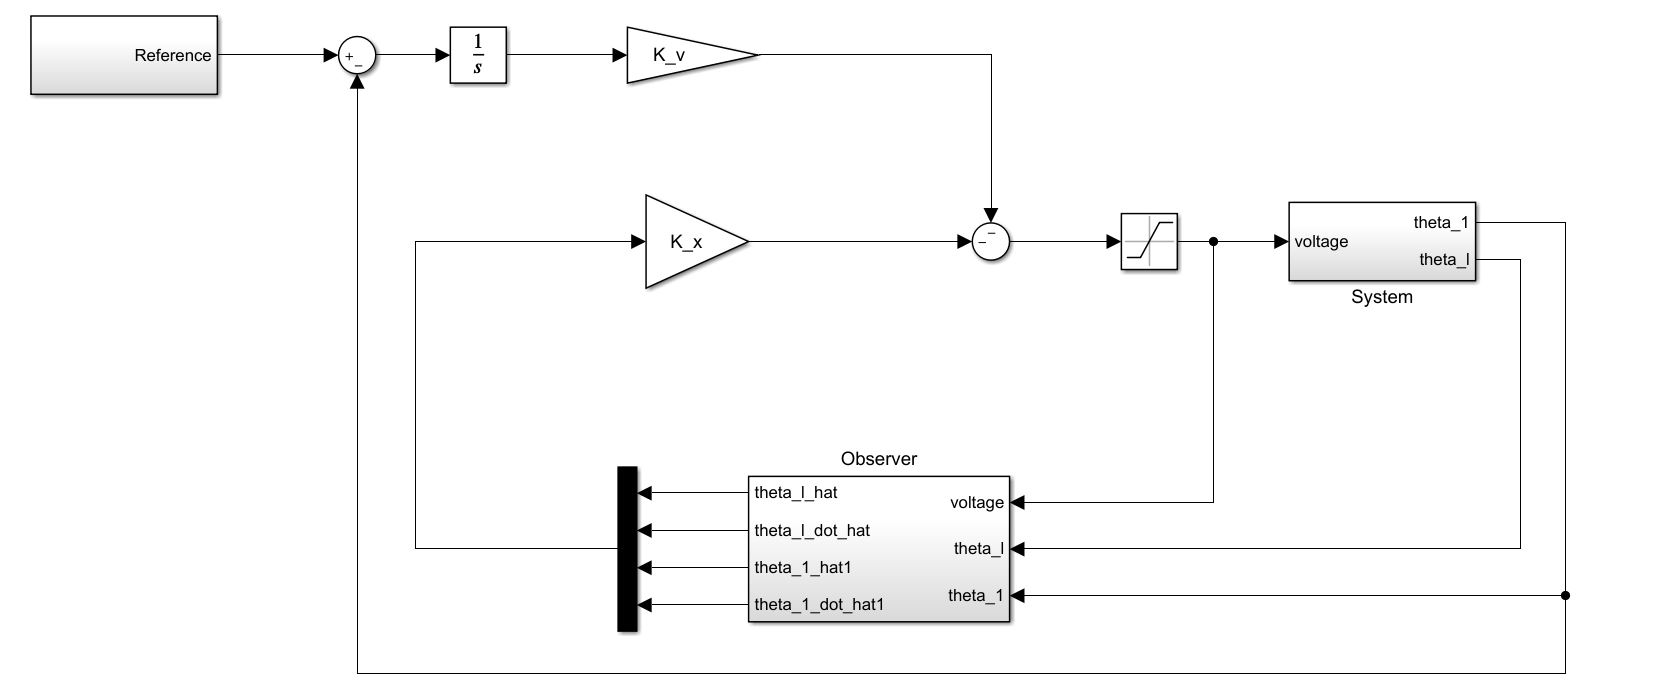
\includegraphics[scale=0.3]{pp_1}
	\caption{block scheme with pole placement and state reconstraction}
	\label{fig:block scheme with pole placement and state reconstraction}
\end{figure*}

\newpage

In figure \ref{fig:block scheme with pole placement and state reconstraction}, the state estimator block represents either the observer or one of the kalman filters. 
At this point we set the poles through the \textit{place} matlab function. In particular we decide to postpone the real poles to speed up the system, whereas concerning the complex ones we just enhance their damping coefficients. At the beginning we thought to turn them into real poles but the resulting control effort was very aggressive and it was not leading any significant improvement to the dynamics. The placed poles and the corresponing gain $K$ computed by the above-mentioned matlab function are written below:
\\\\

\begin{equation}
	PlacedPoles^{T} =
	\begin{bmatrix}
		-20 \\ -50 \\ -40.1*(0.8+\sin(\arccos(0.8))*i) \\ -40.1*(0.8-\sin(\arccos(0.8))*i) \\-10  
	\end{bmatrix}
		K_x^{T} =
	\begin{bmatrix}
		185.9405 \\  3.5059 \\ -125.8645 \\   0.1222
	\end{bmatrix}
	\\
	K_v =
	\begin{bmatrix}
		286.2122
	\end{bmatrix}
\end{equation}

We will provide now the comparison between the configurations made by the same pole placement and the different state estimator. We will do it plotting also the simulation made through our scheme. Doing so we test the reliability of our model with respect the real system.

\begin{figure*}[h]
	\centering
	\begin{subfigure}{0.45\columnwidth}
		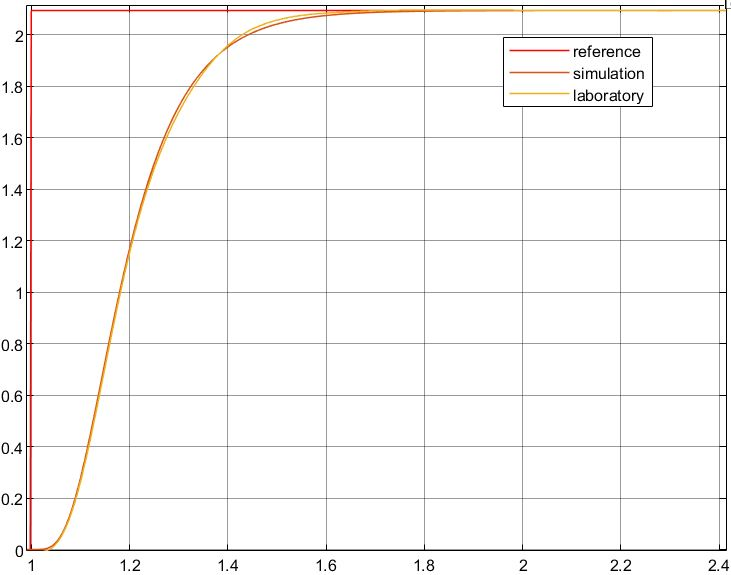
\includegraphics[scale=0.55]{response_pp_1}
		\caption{Position}
	\end{subfigure}
	\begin{subfigure}{0.45\columnwidth}
		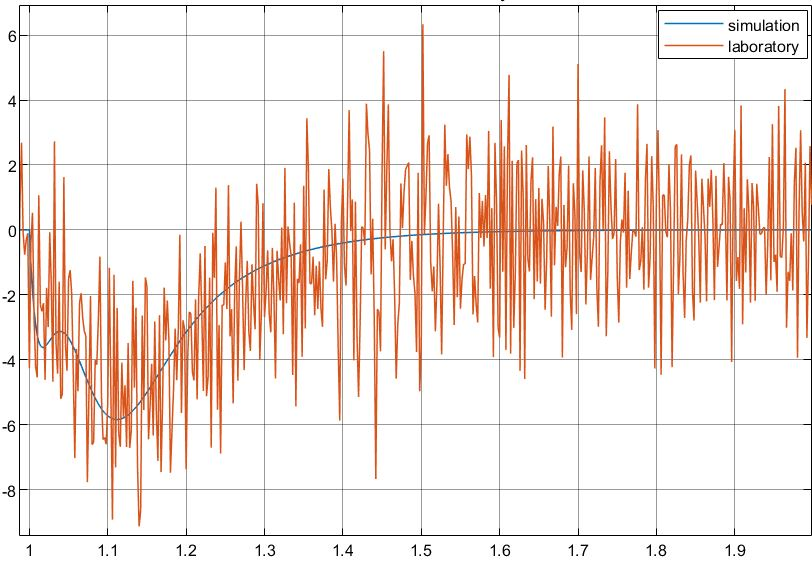
\includegraphics[scale=0.565]{voltage_pp_1}
		\caption{Voltage}
	\end{subfigure}
	\caption{Position step response with full-state observer}
	\label{fig:Position step response with full-state observer}
\end{figure*}

\begin{figure*}[h]
	\centering
	\begin{subfigure}{0.45\columnwidth}
		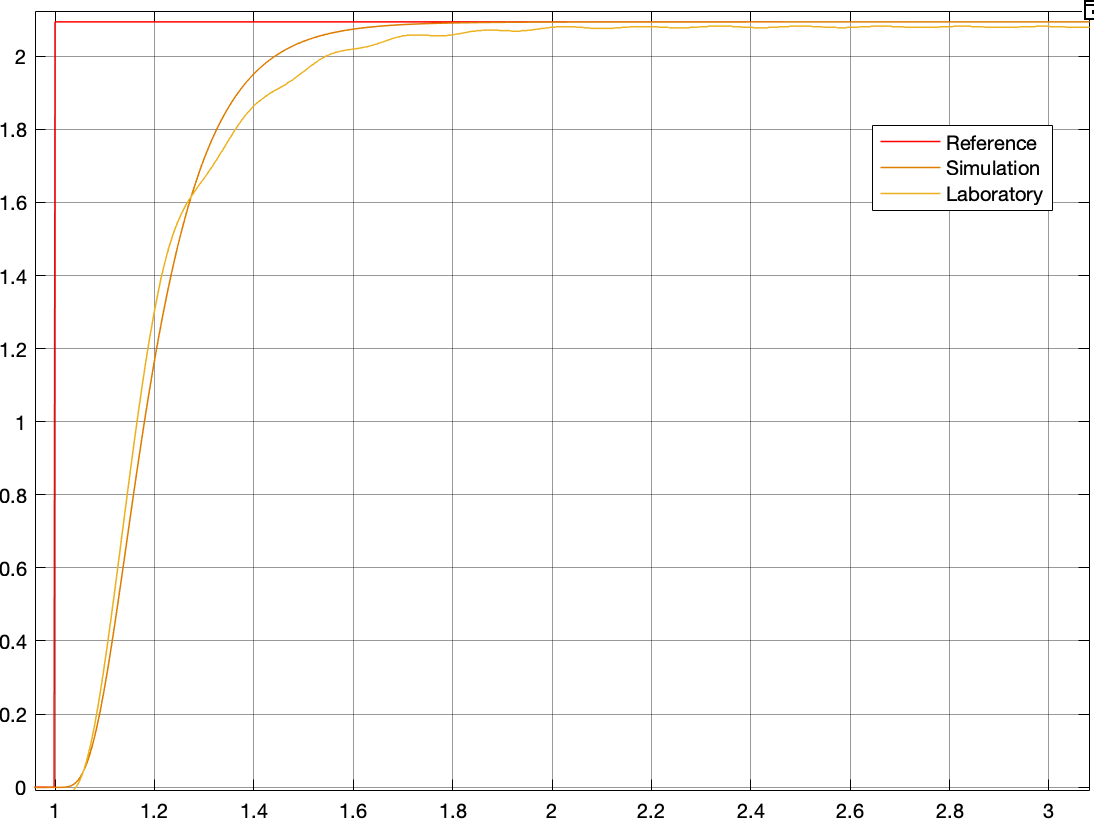
\includegraphics[scale=0.37]{kf1_pp_1}
		\caption{Position}
	\end{subfigure}
	\begin{subfigure}{0.45\columnwidth}
		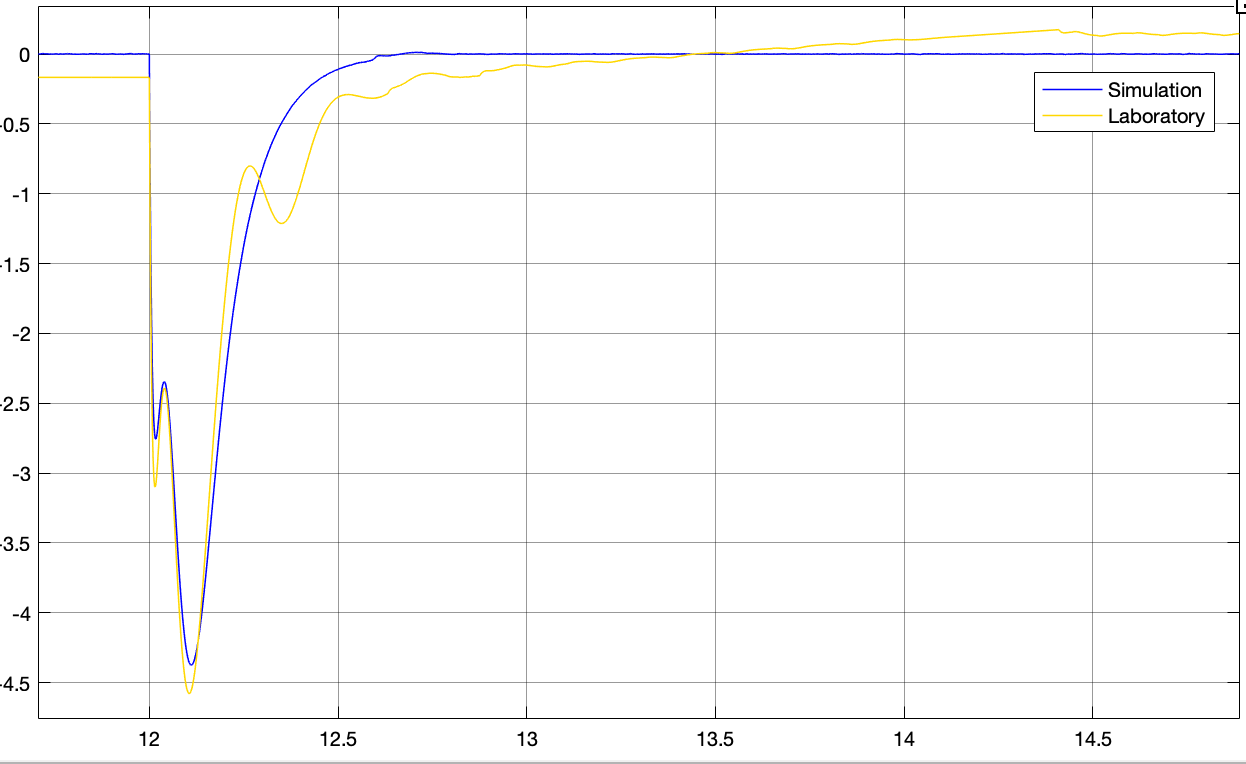
\includegraphics[scale=0.37]{kf1_pp_2}
		\caption{Voltage}
	\end{subfigure}
	\caption{Position step response with full Kalman filter (potentiometer and enconder)}
	\label{fig:Position step response with full Kalman filter}
\end{figure*}

As regards the step response, we can notice as the Kalman filter configuration is not as smooth as the observer one. This might be caused by a small uncertainty that our model has with respect to real system. By the way, both cases are considered acceptable. On the other hand, the kalman filter brings a significant improvement on the control action, resulting to be less noisy due to the filter robustness against the white noises.
We are already satisfied by this performance and we do not need to speed it up, however other solutions will be provided later on with LQG.

\section{2-DOF}
As before, we enlarge the system in order to reach the position reference. The overall enlarged state space system and the closed control loop scheme are the following ones:

\begin{equation}
	\begin{bmatrix}
		\dot{\theta_l} \\
		\ddot{\theta_l} \\
		\dot{\theta_1} \\
		\ddot{\theta_1} \\
		\dot{\theta_2} \\
		\ddot{\theta_2} \\
		\dot{v}
	\end{bmatrix}
	=
	\begin{bmatrix}
		0 &1 & 0 & 0 & 0 & 0 & 0 \\
		-\frac{K_{s_1}}{J_m} & -\frac{B_m}{J_m}-\frac{\eta_m \eta_g k_t k_m {K_g}^2}{R_m J_m}  & \frac{K_{s_1}}{J_m} & 0 & 0 & 0 & 0 \\
		0 & 0 & 0 & 1 & 0 & 0 & 0\\
		\frac{K_{s_1}}{J_1} & 0 & -\frac{K_{s_1}+K_{s_2}}{J_1} & -\frac{B_1}{J_1} & \frac{K_{s_2}}{J_1} & 0 & 0\\
		0 & 0 & 0 & 0 & 0 & 1 & 0 \\
		0 & 0 & \frac{K_{s_2}}{J_2} & 0 & -\frac{K_{s_2}}{J_2} & -\frac{B_2}{J_2} & 0 \\
		0 & 0 & 0 & 0 & 1 & 0 & 0
	\end{bmatrix}
	\begin{bmatrix}
		\theta_l \\
		\dot{\theta_l} \\
		\theta_1 \\
		\dot{\theta_1} \\
		\theta_2 \\
		\dot{\theta_2} \\
		v 
	\end{bmatrix}
	+
	\begin{bmatrix}
		0 \\
		\frac{\eta_m \eta_g k_t K_g}{R_m J_m} \\
		0 \\
		0 \\
		0 \\
		0 \\
		0 
	\end{bmatrix}
	V
 \end{equation}


\begin{figure*}[h]
	\centering
	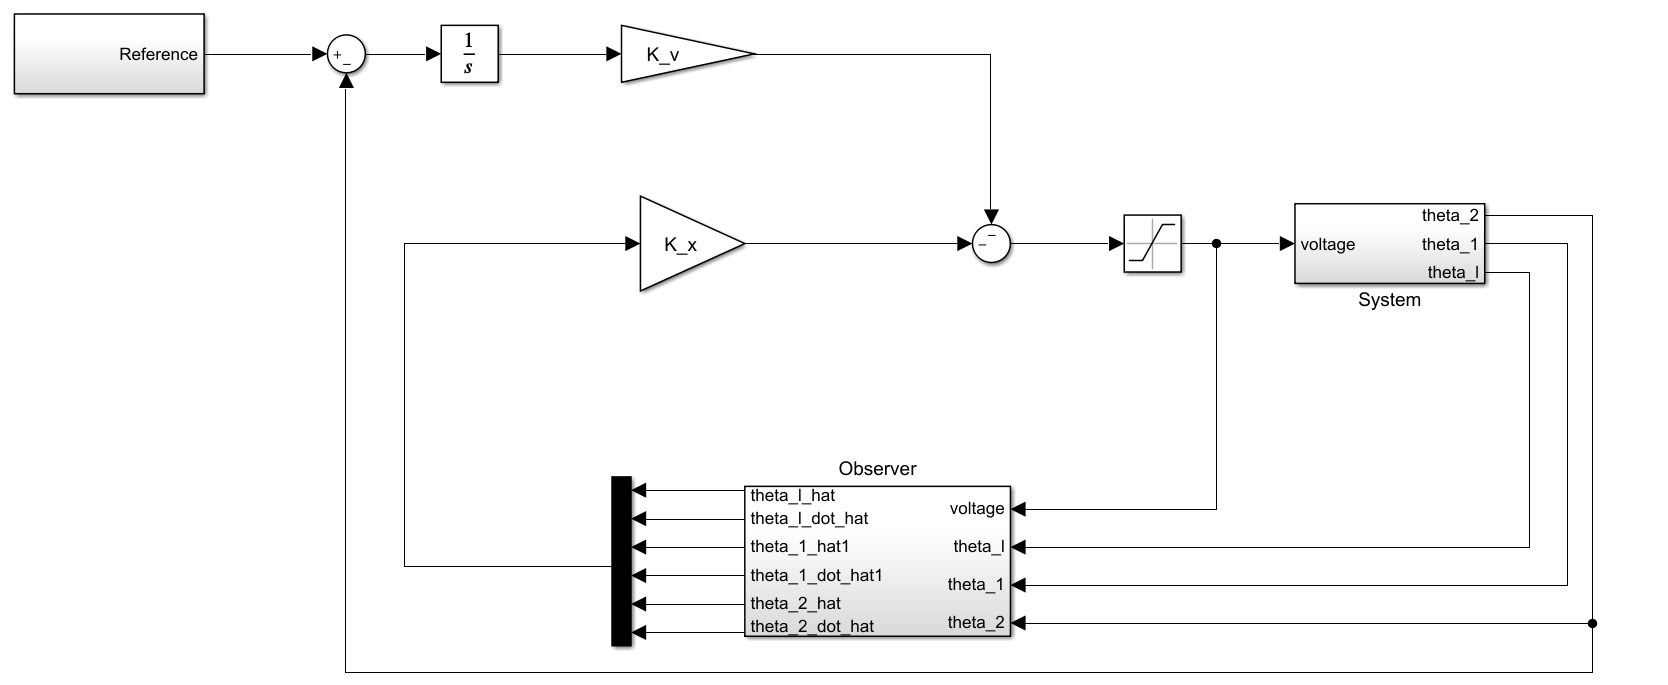
\includegraphics[scale=0.3]{pp_2}
	\caption{Block scheme with pole placement and state reconstruction}
\end{figure*}

Also in this case, we decide not to force the complex poles to real ones, but we just rise their damping coefficients. Below, it is possible to see where we placed the new poles of the system and the gain vector that lets us do it.

\begin{equation}
	PlacedPoles^{T} =
	\begin{bmatrix}
		-20 \\ -30 \\ -24.5*(0.6+\sin(\arccos(0.6))*i) \\ -24.5*(0.6-\sin(\arccos(0.6))*i) \\
		-61.9*(0.2+\sin(\arccos(0.2))*i) \\ -61.9*(0.2-\sin(\arccos(0.2))*i) \\ -10
	\end{bmatrix}
	K_x^{T} =
	\begin{bmatrix}
		68.1752  \\  1.1393 \\ -71.9542 \\   0.0150 \\  30.2715  \\  0.5489
	\end{bmatrix}
	\\
	K_v =
	\begin{bmatrix}
		110.9516
	\end{bmatrix}
\end{equation}

\begin{figure*}[h]
	\centering
	\begin{subfigure}{0.5\columnwidth}
		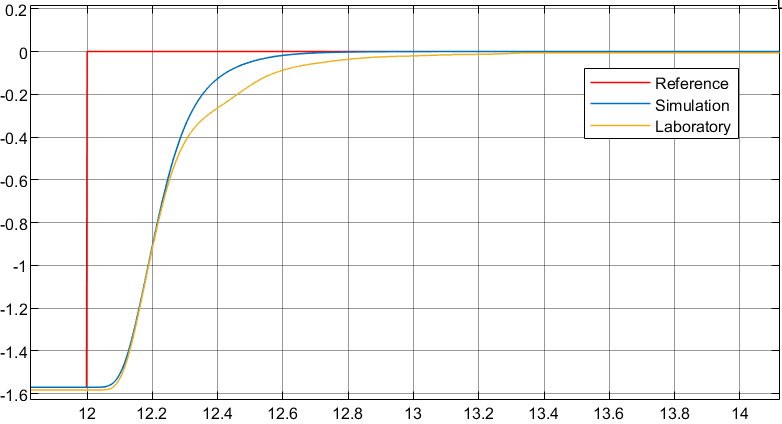
\includegraphics[scale= 0.37]{response_pp_2}
		\caption{Position}
	\end{subfigure}
	\begin{subfigure}{0.45\columnwidth}
		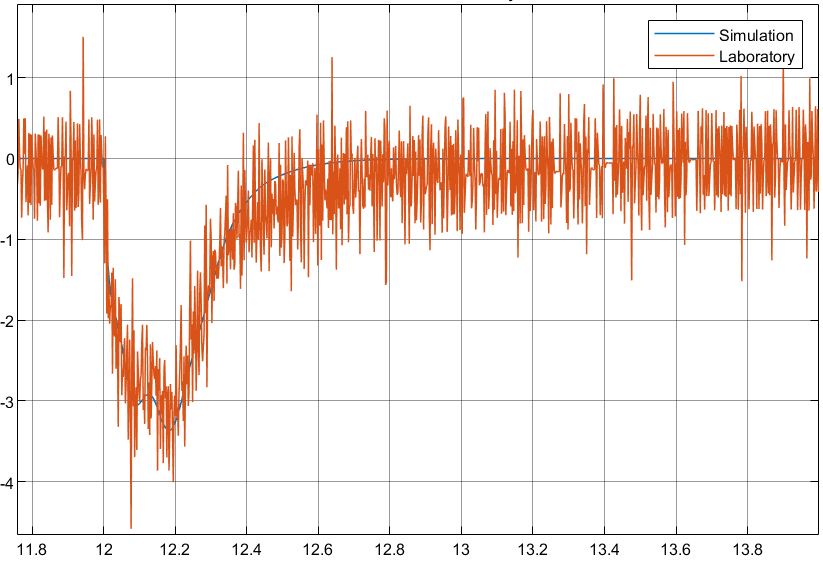
\includegraphics[scale=0.25]{voltage_pp_2}
		\caption{Voltage}
	\end{subfigure}
	\caption{position step response with full-state observer}
\end{figure*}

\begin{figure*}[h]
	\centering
	\begin{subfigure}{0.5\columnwidth}
		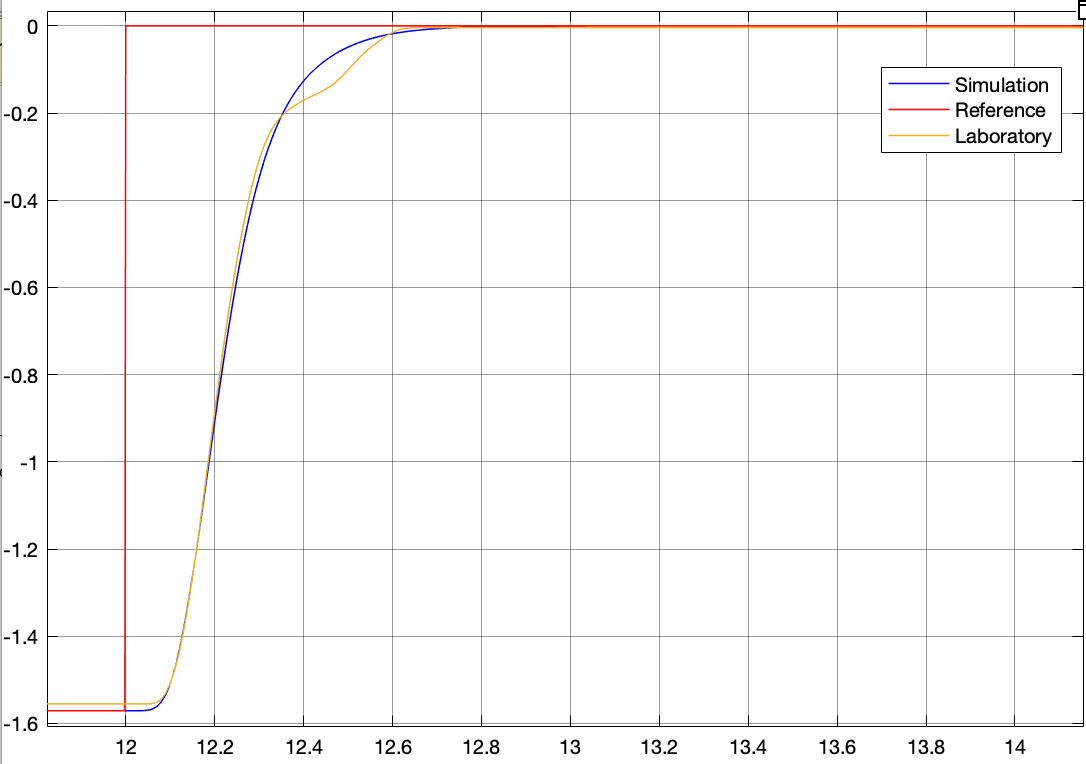
\includegraphics[scale= 0.37]{2_kf1_1}
		\caption{Position}
	\end{subfigure}
	\begin{subfigure}{0.45\columnwidth}
		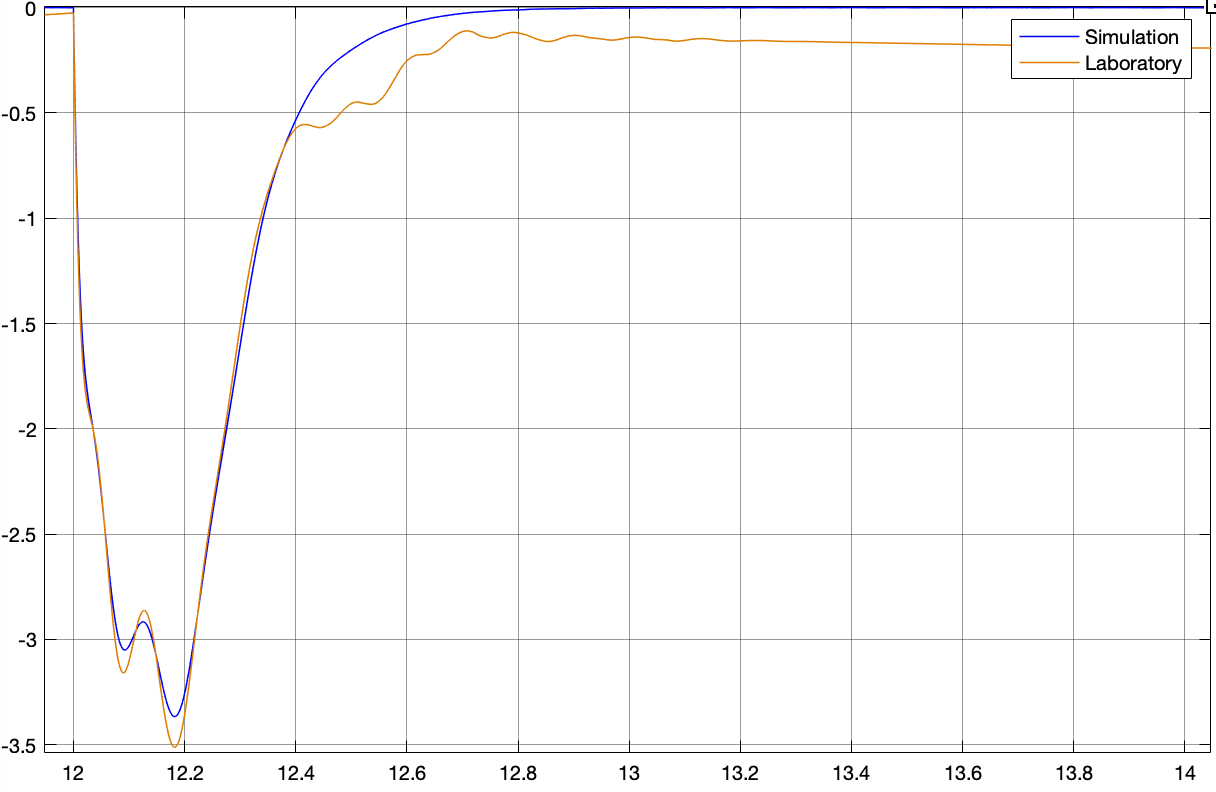
\includegraphics[scale=0.37]{2_kf1_2}
		\caption{Voltage}
	\end{subfigure}
	\caption{Position step response with full Kalman filter (potentiometer and two enconders}
\end{figure*}

\begin{figure*}[h]
	\centering
	\begin{subfigure}{0.5\columnwidth}
		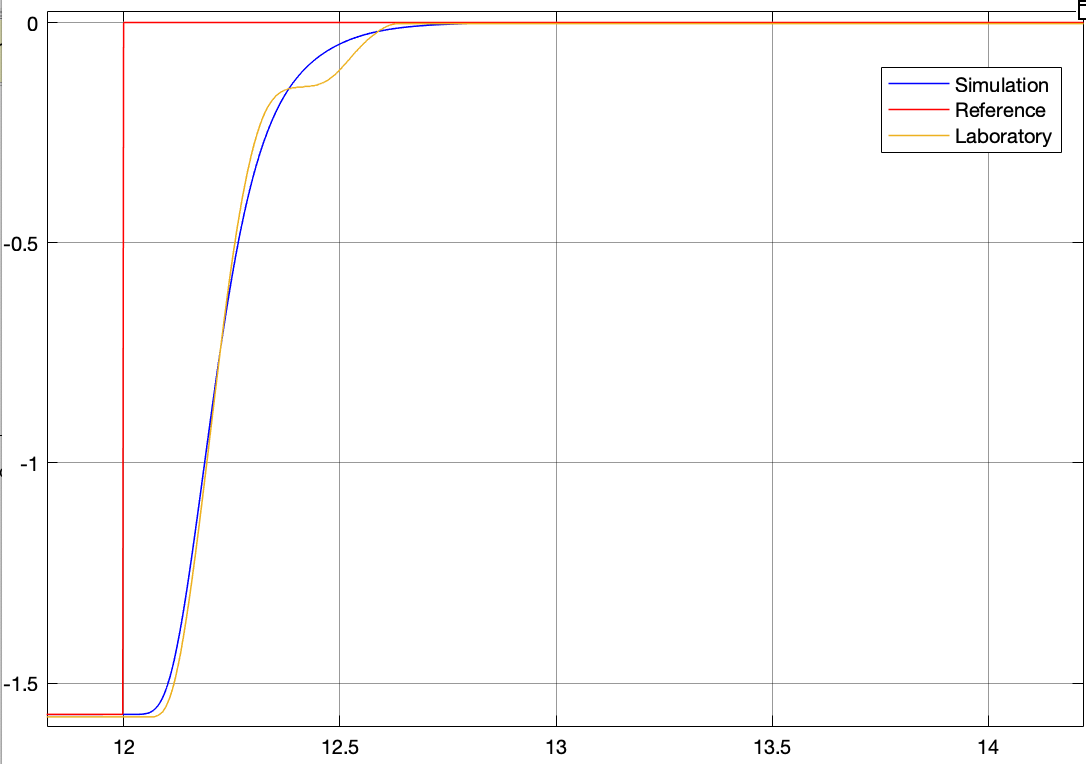
\includegraphics[scale= 0.37]{2_kf2_1}
		\caption{Position}
	\end{subfigure}
	\begin{subfigure}{0.45\columnwidth}
		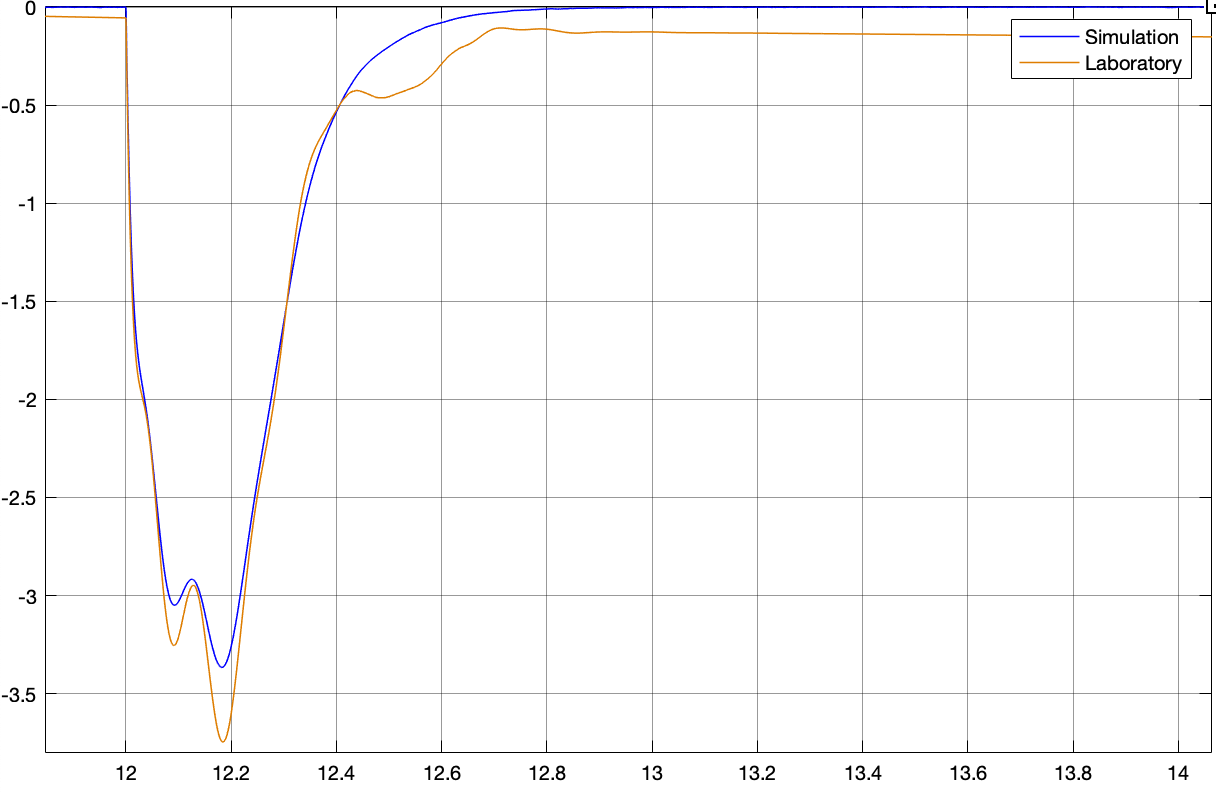
\includegraphics[scale=0.37]{2_kf2_2}
		\caption{Voltage}
	\end{subfigure}
	\caption{Position step response with Kalman filter (second mass enconder only)}
\end{figure*}

